\documentclass[11pt, titlepage]{article}
\usepackage{amsmath,amsthm,amssymb}
\usepackage{hyperref, pgf, tikz}
\usepackage{fancyhdr}
\usetikzlibrary{arrows}
\usepackage[margin=1.25in]{geometry}
\usepackage{graphicx}                     
\pagestyle{fancy}
\usepackage{array}
%\usepackage{wrapfig}

\lhead{Lab \#02}
\rhead{\thepage}
\cfoot{}

\title{\Huge{Projectile Motion: The Ballistic Pendulum} \\ \ \\ \huge Lab \#02}
\author{\Large{Alon Levin} \\ \emph{Lab Partner: Avery Karlin}}
\date{\today}
\begin{document}

\maketitle

\begin{center}
\LARGE Projectile Motion: The Ballistic Pendulum
\end{center}

\section*{Objective}
The objectives of this lab are to use a ballistic penduluma \& the laws of conservation (of linear momentum and energy) to determine the initial velocity of a projectile, to describe the components of motion \& how they are used in the determination of the velocity of a projectile with range-fall measurements, and to tell how the range of a projectile varies with the angle of projection.

\section*{Introduction}
\subsection*{The Ballistic Pendulum}
The ballistic pendulum, in its crudest form, is an apparatus used to measure the initial velocity of a horizontally projected object acted on by a spring by determining the height of the pendulum into which the projectile is fired. To facilitate the experiment, a spring gun is used to fire a small metal ball into a hollow pendulum, which then stops at its highest point by the use of a catch mechanism.

By measuring the difference in height between the pendulum system's starting and final positions with respect to its center of gravity, it is possible to compute the initial velocity of the projectile through the use of the laws of Conservation of Linear Momentum and Conservation of Mechanical Energy, assuming that rotaional considerations are to be neglected. 

\subsubsection*{Calculations}
Assume that a projectile of mass $m$ is fired from the spring gun with an initial velocity $v_{x_o}$ into a stationary pendulum of mass $M$ and becomes embedded in it. Horizontal momentum is conserved (as all other forces are perpendicular to the direction of motion), and to a good approximation applies over the time interval of the collision --- thus, it can be taken that linear momentum is identical immediately before and after the collision. The velocity of the pendulum bob is initally $0$; the combined system has a velocity of magnitude $V$ just after the collision. From this information, we get the following equation equating the linear momentum immediately before the collision and immediately after the collision:
\begin{equation} \label{eq:1}
mv_{x_o} = (m+M)V
\end{equation}

After the collision, the pendulum-projectile system swings upward, indicating that the system's momentum is no longer preserved. As soon as it reaches its maximum vertical distance the vertical displacement $h$ could be measured thanks to the catch mechanism on the pendulum. Mechanical energy is conserved, so the increase in potential energy witnessed by the vertical displacement must be equal to the kinetic energy of the system immediately following collision if friction and drag are to be neglected. Thus, we get the following equation:
\begin{equation} \label{eq:2}
\frac{1}{2}(m+M)V^2 = (m+M)gh
\end{equation}
Solving Eq. \ref{eq:2} for $V$, we obtain
\begin{equation} \label{eq:3}
V = \sqrt{2gh}
\end{equation}
which we can then substitute into Eq. \ref{eq:1} to solve for $v_{x_o}$, yieding
\begin{equation} \label{eq:4}
v_{x_o} = \frac{m+M}{m}\sqrt{2gh}
\end{equation}

\subsection*{Parabolic Projectile Motion}
\subsubsection*{Calculation of Initial Velocity from Range-Fall Measurements}
If a projectile were to be fired horizontally with intial velocity $v_{x_o}$ from a height $y$, it would travel in an arc a horizontal distance (or \emph{range}) $x$ while falling a vertical distance $y$. Because it is fired horizontally, initial vertical velocity  $v_{y_o} = 0$. However, it increases over time because acceleration due to gravity $a_y = g$ is positive downward. Using this information, we get the following components for the motion of the projectile:
\begin{equation} \label{eq:5}
x = v_{x_o}t
\end{equation}
\begin{equation} \label{eq:6}
y = \frac{1}{2}gt^2
\end{equation}
Eliminating $t$ from Eqs. \ref{eq:5} \& \ref{eq:6} and solving for $v_{x_o}$, we arrive at the following equation, neglecting air resistance:
\begin{equation} \label{eq:7}
v_{x_o} = \sqrt{\frac{gx^2}{2y}} = (\frac{g}{2y})^\frac{1}{2}x
 \end{equation}
 
\subsubsection*{Range Dependence on Angle of Projection}
The components of the initial velocity of a projectile fired at a general angle $\theta$ have magnitudes of
$$v_{x_o} = v_o\cos\theta$$
\begin{equation} \label{eq:8}
v_{y_o} = v_o\sin\theta
\end{equation}
At the top of the arc path, $v_y = 0$, and since
$$v_y = v_{y_o} - gt = v_0\sin\theta - gt$$
we have
$$v_o\sin\theta - gt_m = 0$$
or
\begin{equation} \label{eq:9}
t_m = \frac{v_o\sin\theta}{g}
\end{equation}
where $t_m$ is the time needed for the projectile to reach maximum height $y_m$. If the projectile returns to its starting elevation $y=0$, the total time of flight $t$ is
\begin{equation} \label{eq:10}
t = 2t_m = \frac{2v_o\sin\theta}{g}
\end{equation}

During the time $t$ the projectile travels a range R in which 
$$R = v_{x_o}t = \frac{2{v_o}^2\sin\theta cos\theta}{g}$$
or, when rewritten using the trigonometric identity $2\sin\theta \cos\theta = \sin(2\theta)$,
\begin{equation} \label{eq:11}
R = \frac{{v_o}^2\sin(2\theta)}{g}
\end{equation}
Thus, we see that the range depends on the angle of projection. By observation, it is understood that $R_{max}$ occurs when $\sin(2\theta) = 1$, and since $\sin90^\circ = 1$ by comparison we obtain $\theta = 45^\circ$. Hence, a projectile has a maximum range for $\theta = 45^\circ$ and
\begin{equation} \label{eq:12}
R_{max} = \frac{{v_o}^2}{g}
\end{equation}

\pagebreak
\section*{Procedure}
After collecting initial measurements and setting up the apparatus properly (see Fig. \ref{fig:setup}), the ball is fired into the freely hanging stationary pendulum; the notch at which the catch-mechanism stops the pendulum's motion should be noted. Repeat this procedure for four more trials, and then find the height of the notch most closely corresponding to the average measure of the height based on the five trials. Using this data, the initial velocity could be calculated using Eq. \ref{eq:4}.

To modify the setup for parabolic projectile motion, the pendulum should be removed and set aside. Position the apparatus on a raised platform with the end of the base touching the edge, and fire the ball from the spring gun, noting how far it lands from the starting point. Fire the ball four more times and measure the range that it traveled each time. Using the average range and the height from which the ball was fired, the initial velocity could be calculated using Eq. \ref{eq:7}.

The apparatus should be raised on an incline to create the angle required to determine the effect of angle of projection on the range. Fire the ball from predetermined angles (with a few trials per angle) and note the average range for each angle of projection used. Plot the range versus the angle of projection, and draw a smooth best-fit curve. Use this graph to determine the angle required to obtain maximum range.
\begin{figure}[!ht]
\centering
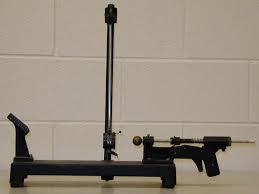
\includegraphics[scale=1.5, angle=0]{lab02.jpg}
\caption{Setup used for this experiment \label{fig:setup}}
\end{figure}

\pagebreak
\section*{Data}
Height of pointer with pendulum catch in closest-to-average notch number:
$$h_2 = 0.094 m$$
Height of pointer with pendulum freely suspended:
$$ h_1 = 0.056 m$$
Difference in heights:
$$h = h_2 - h_1 = 0.038 m$$
Mass of ball:
$$m = 0.0691 kg$$
Mass of pendulum, including bob and support:
$$M = 0.28 kg$$
\begin{center}
\begin{tabular}
{|m{7em}|m{7em}|}
\hline
Trials & Notch Number of Pendulum Catch \\
\hline
1 & 12\\
\hline
2 & 15\\
\hline
3 & 19\\
\hline
4 & 19\\
\hline
5 & 23\\
\hline
Average & 17.6\\
\hline
\end{tabular}
\end{center}
Initial horizontal velocity A, calculated:
$$v_{x_o} = 4.362 m/s$$

\pagebreak
\noindent Vertical distance of fall:
$$y = 0.5 m$$
\begin{center}
\begin{tabular}
{|m{7em}|m{7em}|}
\hline
Trials & Range\\
\hline
1 & 2.2\\
\hline
2 & 2.155\\
\hline
3 & 2.105\\
\hline
4 & 2.123\\
\hline
5 & 2.125\\
\hline
Average & 2.1416\\
\hline
\end{tabular}
\end{center}
Initial horizontal velocity B, calculated:
$$v_{x_o} = 6.708 m/s$$
Percent difference between results of parts A and B:
$$\text{Diff} = 34.97\%$$
Average initial velocity, based on results of parts A and B:
$$v_o = 5.535 m/s$$
\begin{center}
\begin{tabular}
{|m{7em}|m{7em}|m{7em}|}
\hline
Angle of projection & Average range & Calculated range\\
\hline
$20^o$ & 3.23 & 2.01\\
\hline
$30^o$ & 3.82 & 2.70\\
\hline
$40^o$ & 4.08 & 3.08\\
\hline
$45^o$ & 4.31 & 3.12\\
\hline
$50^o$ & 4.12 & 3.08\\
\hline
$60^o$ & 3.64 & 2.70\\
\hline
$70^o$ & 3.44 & 2.01\\
\hline
\end{tabular}
\end{center}
Angle of projection for maximum range from graph:
$$ \theta = 45.58^\circ$$
\pagebreak
\section*{Discussion}
\subsection*{Sample Calculations}
$$v_{x_o} = \frac{0.0691+0.28}{0.0691}\sqrt{2\ast9.81\ast0.038} = 4.362 m/s$$
$$v_{x_o} = (\frac{9.81}{2\ast.5})^\frac{1}{2}\ast2.1416 = 6.708 m/s$$
$$\text{Diff} = \frac{6.708-4.362}{6.708}\ast100\% = 34.97\%$$
\subsection*{Analysis}
Although there was a high difference between the values for $v_{x_o}$ calculated for parts A and B, the primary cause of this error could come from inaccurate measurement of the range. There are several reasons for which this inaccuracy could have come about, including shifting of the landing paper under the carbon paper and improper meterstick placement. This, in turn, affects the results of the third portion of the lab, as $v_o$ was calculated as the average of $v_{x_o}$ for parts A and B. However, this does not affect the value for the expected angle of projection for maximum range:
\begin{figure}[!ht]
\centering
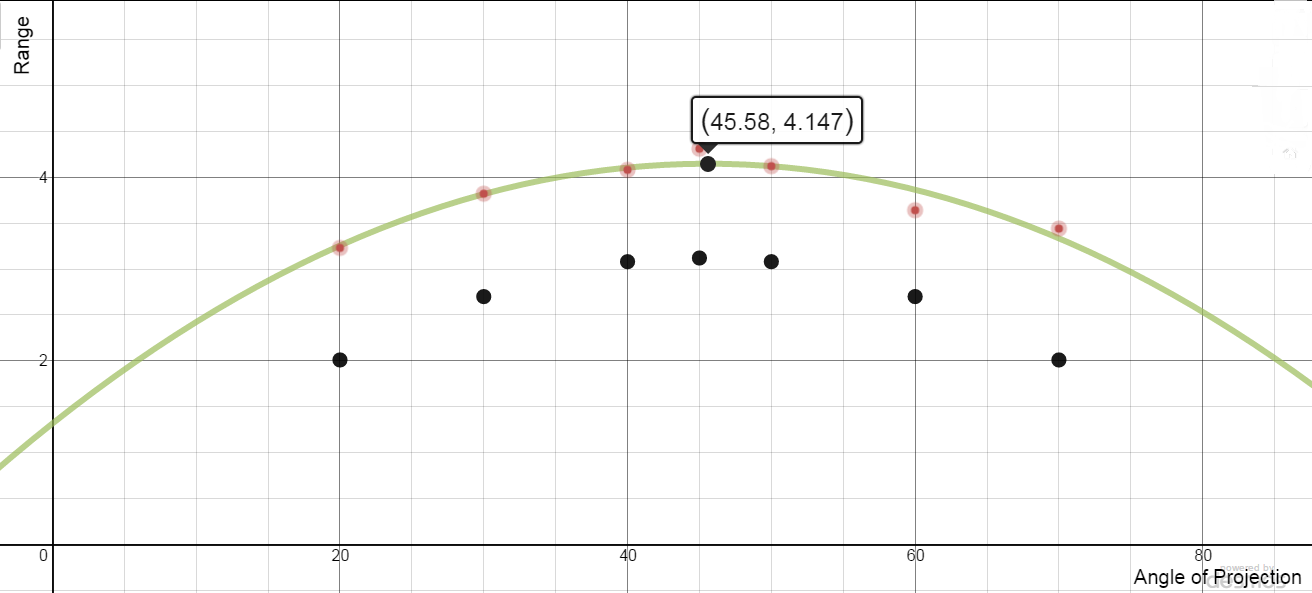
\includegraphics[scale=.4, angle=0]{lab02_graph.png}
\caption{Range vs Angle of Projection \label{fig:graph}}
\end{figure}

\noindent As shown in Fig. \ref{fig:graph}, the optimal angle is still roughly $45^\circ$, even despite the error in measurements.

\section*{Conclusion}
As the angle increased from $20^\circ$ to $45^\circ$, the range of the fired projectile increased from $3.32 m \text{to} 4.31 m$; however, as the angle continued increasing from $45^\circ$ to $70^\circ$, the range decreased from $4.31 m \text{to} 3.44 m$. This indicates that the maximum range attained by a projectile occurs when it is fired at an angle of $45^\circ$.
\end{document}